%
% The first command in your LaTeX source must be the \documentclass command.
\documentclass[sigconf,nonacm,natbib=false]{acmart}
\settopmatter{printacmref=true}

\PassOptionsToPackage{ngerman}{babel}

\usepackage[style=ACM-Reference-Format,backend=biber,sorting=none]{biblatex}
\addbibresource{references.bib}

%
% defining the \BibTeX command - from Oren Patashnik's original BibTeX documentation.
\def\BibTeX{{\rm B\kern-.05em{\sc i\kern-.025em b}\kern-.08emT\kern-.1667em\lower.7ex\hbox{E}\kern-.125emX}}
    
% Rights management information. 
% This information is sent to you when you complete the rights form.
% These commands have SAMPLE values in them; it is your responsibility as an author to replace
% the commands and values with those provided to you when you complete the rights form.
%
% These commands are for a PROCEEDINGS abstract or paper.
\copyrightyear{2018}
%\acmYear{2018}
%\setcopyright{acmlicensed}
%\acmConference[Woodstock '18]{Woodstock '18: ACM Symposium on Neural Gaze Detection}{June 03--05, 2018}{Woodstock, NY}
%\acmBooktitle{Woodstock '18: ACM Symposium on Neural Gaze Detection, June 03--05, 2018, Woodstock, NY}
%\acmPrice{15.00}
%\acmDOI{10.1145/1122445.1122456}
%\acmISBN{978-1-4503-9999-9/18/06}

%
% These commands are for a JOURNAL article.
%\setcopyright{acmcopyright}
%\acmJournal{TOG}
%\acmYear{2018}\acmVolume{37}\acmNumber{4}\acmArticle{111}\acmMonth{8}
%\acmDOI{10.1145/1122445.1122456}

%
% Submission ID. 
% Use this when submitting an article to a sponsored event. You'll receive a unique submission ID from the organizers
% of the event, and this ID should be used as the parameter to this command.
%\acmSubmissionID{123-A56-BU3}

%
% The majority of ACM publications use numbered citations and references. If you are preparing content for an event
% sponsored by ACM SIGGRAPH, you must use the "author year" style of citations and references. Uncommenting
% the next command will enable that style.
%\citestyle{acmauthoryear}

%
% end of the preamble, start of the body of the document source.
\begin{document}

%
% The "title" command has an optional parameter, allowing the author to define a "short title" to be used in page headers.
\title{Mögliche Probleme bei
der Anwendung von
Deep-Learning}
\subtitle{Poster Paper}

%
% The "author" command and its associated commands are used to define the authors and their affiliations.
% Of note is the shared affiliation of the first two authors, and the "authornote" and "authornotemark" commands
% used to denote shared contribution to the research.
\author{Bennet Bleßmann}
\authornote{Todo}
\email{bennet.blessmann@stu.uni-kiel.de}

%
% The abstract is a short summary of the work to be presented in the article.
\begin{abstract}
When applying Deep-Learning one has to lookout for some obvious and some hidden 
Problems which may occur in any of the development phases.
\end{abstract}

%
% The code below is generated by the tool at http://dl.acm.org/ccs.cfm.
% Please copy and paste the code instead of the example below.
%
\begin{CCSXML}
<ccs2012>
<concept>
<concept_id>10011007.10011074.10011092.10011782.10011813</concept_id>
<concept_desc>Software and its engineering~Genetic programming</concept_desc>
<concept_significance>500</concept_significance>
</concept>
<concept>
<concept_id>10011007.10011074.10011075.10011078</concept_id>
<concept_desc>Software and its engineering~Software design tradeoffs</concept_desc>
<concept_significance>300</concept_significance>
</concept>
<concept>
<concept_id>10011007.10011074.10011075.10011079</concept_id>
<concept_desc>Software and its engineering~Software implementation planning</concept_desc>
<concept_significance>300</concept_significance>
</concept>
<concept>
<concept_id>10011007.10011074.10011099.10011693</concept_id>
<concept_desc>Software and its engineering~Empirical software validation</concept_desc>
<concept_significance>300</concept_significance>
</concept>
<concept>
<concept_id>10002978</concept_id>
<concept_desc>Security and privacy</concept_desc>
<concept_significance>300</concept_significance>
</concept>
<concept>
<concept_id>10010147.10010257</concept_id>
<concept_desc>Computing methodologies~Machine learning</concept_desc>
<concept_significance>300</concept_significance>
</concept>
<concept>
<concept_id>10010520.10010521.10010542.10010294</concept_id>
<concept_desc>Computer systems organization~Neural networks</concept_desc>
<concept_significance>300</concept_significance>
</concept>
<concept>
<concept_id>10003120</concept_id>
<concept_desc>Human-centered computing</concept_desc>
<concept_significance>100</concept_significance>
</concept>
<concept>
<concept_id>10010405.10010455</concept_id>
<concept_desc>Applied computing~Law, social and behavioral sciences</concept_desc>
<concept_significance>100</concept_significance>
</concept>
</ccs2012>
\end{CCSXML}

\ccsdesc[500]{Software and its engineering~Genetic programming}
\ccsdesc[300]{Software and its engineering~Software design tradeoffs}
\ccsdesc[300]{Software and its engineering~Software implementation planning}
\ccsdesc[300]{Software and its engineering~Empirical software validation}
\ccsdesc[300]{Security and privacy}
\ccsdesc[300]{Computing methodologies~Machine learning}
\ccsdesc[300]{Computer systems organization~Neural networks}
\ccsdesc[100]{Human-centered computing}
\ccsdesc[100]{Applied computing~Law, social and behavioral sciences}

\ccsdesc[500]{Computer systems organization~Embedded systems}
\ccsdesc[300]{Computer systems organization~Redundancy}
\ccsdesc{Computer systems organization~Robotics}
\ccsdesc[100]{Networks~Network reliability}

%
% Keywords. The author(s) should pick words that accurately describe the work being
% presented. Separate the keywords with commas.
\keywords{datasets, neural networks, privacy, human-centered computing}

%
% A "teaser" image appears between the author and affiliation information and the body 
% of the document, and typically spans the page. 
%\begin{teaserfigure}
%  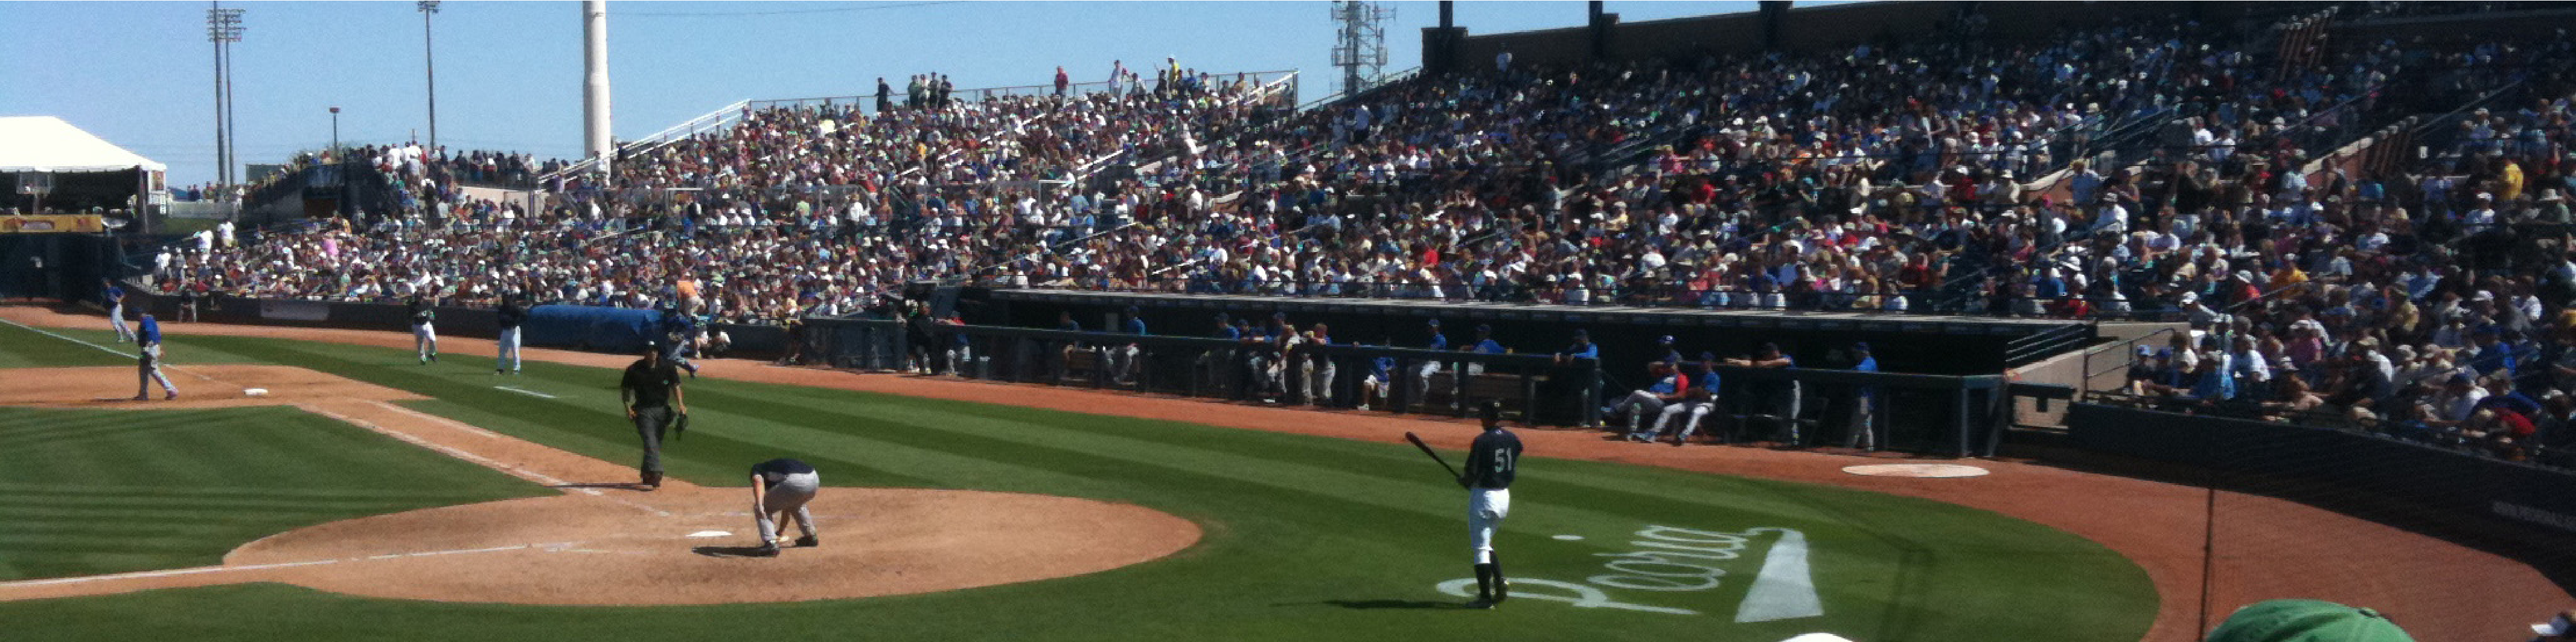
\includegraphics[width=\textwidth]{sampleteaser}
%  \caption{Seattle Mariners at Spring Training, 2010.}
%  \Description{Enjoying the baseball game from the third-base seats. %Ichiro Suzuki preparing to bat.}
%  \label{fig:teaser}
%\end{teaserfigure}


%
% This command processes the author and affiliation and title information and builds
% the first part of the formatted document.
\maketitle

\section{Introduction}

This Paper will at first describe possible Problems when applying Deep-Learning technologies and their possible effects. The Problems will be grouped based on the development phase we expect them to be rooted in. After the Problems have been described it will if possible present general solution to said Problems or otherwise it might give solutions for special cases. It shall me noted that some of these Problems apply to software development of any kind.

\section{Definitions}

\subsection{A Problem}
A Problem is anything which may result in unwanted negative effects of any kind.

\subsection{The Phases of Development}
For the Phases of development this paper will assume the following five stages similar to those found in the Waterfall model.
In real world application these phases might occur in parallel or multiple times or not at all.

The first Phase of Development is the phase of discovering and evaluating the Projects requirements, usually these might be constrained by a customers wishes and budget.

The second Phase of Development is the planning Phase where based on the result of the first Phase will be decided on the general structure of the Project.

The third Phase of Development is the Phase of actually implementing the Projects Plan and requirements.

The fourth Phase is where we have a larger divergent from the waterfall model as this is the Phase where the Algorithm will be trained, this is not a phase found in typical software development.

The last Phase is the Phase of Usage and Maintenance where the Product will be applied in the world and needs to be maintained.

\section{Problems}

\subsection{Requirements Phase}
Problems occurring and not being acknowledged in this phase
might be hard to resolve at a later stage as this phase presents the 
foundation for all further phases.

\paragraph{Vague Goal}
Problems in this Phase include a vaguely defined goal,
for construction a selection algorithm this might be 
an undefined fairness metric resulting in an algorithm considered unfair.

\paragraph{Morally acceptability}
Another Problem which might be less concrete might be the consideration if an algorithms should be developed at all,
as an algorithm might be possible but morally unwanted.

\paragraph{Economical incentive}
Probably the most tangible Problem is the collision of moral and ethics with economics, given the current economic structure it would be unreasonable in most circumstances to produce a socially beneficial algorithm without any directly visible economic benefit for any participating party, on the other hand it might be of interest to produce an ethical, morally or socially problematic algorithm for ones economically benefit. 

\paragraph{Evaluation of Consequences}
% Fehelende Folgenabschätzung

\subsection{Planning Phase}
Intro

\paragraph{Incorrect Model}
\paragraph{Insufficient Safety Considerations}

\subsection{Development Phase}
Intro
\paragraph{Missing Dokumentation}
% Mangelnde Dokumentation (Annahmen, Funktionsweise etc.)

\paragraph{Missing Data Protection}
% Mangelder/Vernachlässigter Datenschutz

\subsection{Training Phase}
Into
\paragraph{Insufficient Representation of Reality}
% Unzureichende Abbildung der Realitzät durch Trainingsdaten
\paragraph{Dirty Data}
% Unreine Daten
\paragraph{Irrelevant Data}
% Irrelevante Daten
\paragraph{Contaminated Data}
% Korrekte aber unpassende Daten (wiederspiegeln von Rassismus in der Gesselschaft etc.)

\subsection{Deployment/Maintenance Phase}
% Fehlende Nachvollziehbarkeit
% Unvorhergesehene Einflüsse
% Mangelndes Vertrauen in Technick (Bevölkerung)
% Unvorhergesehene Folgen (Requirement Phase 4?)
% Unklare Haftung (Nutzer, Produzent, Entwickler ?)


%
% The acknowledgments section is defined using the "acks" environment (and NOT an unnumbered section). This ensures
% the proper identification of the section in the article metadata, and the consistent spelling of the heading.
\begin{acks}
To Daniela Stollberg for helping to check the Paper for Grammatical and Syntactical errors.
\end{acks}

%
% The next two lines define the bibliography style to be used, and the bibliography file.

\nocite{*}

\printbibliography

% 
% If your work has an appendix, this is the place to put it.
\appendix

\end{document}
